\section{Introduction}

\begin{figure}[h]
	\centering
	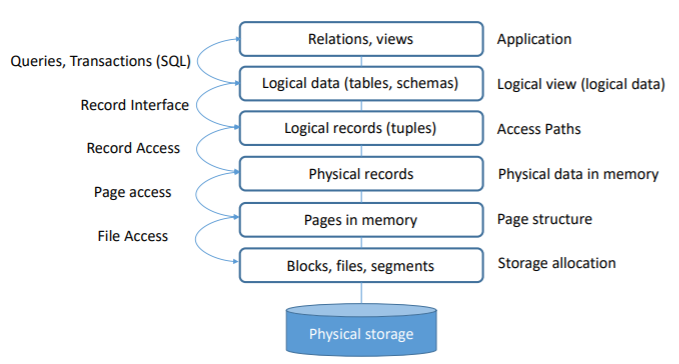
\includegraphics[scale=0.8]{images/00-arch.PNG}
	\caption{Architecture of a database.}
	\label{fig:arch}
\end{figure}

\paragraph{Database Management System (DBMS)}
Tool that helps develop and run data-intensive applications. A DBMS pushes the complexity of dealing with the data (storage, processing, consistency) to the database rather than to the program.

\paragraph{Relational Database}
%TODO
% tuples have no order - delete and insert can mix up tuples in data storage

\paragraph{Physical Data Independence}
The ability to modify the physical schema (to improve performance) without causing the application programs to be rewritten i.e. without affecting the conceptual / external view of the data. The database hides how the data is actually stored persistently and represented in memory.

\paragraph{Logical Data Independence}
The ability to modify the logical schema without causing application programs to be rewritten. A database allows to build views over the schema s.t. different logical interpretations of the same data are possible. E.g. adding a new column to one user will not change the outcome for another user.

\paragraph{Declarative Language}
SQL is a declarative language and specifies how the result looks like while describing the tuples that should be part of it. A DL does not specify how to get to the result (i.e. no control flow, only logic of a computation - what, not how). With this, the DB can optimize queries.

\paragraph{Query Processing / Relational Algebra}
%TODO all the operators


\paragraph{Query Optimization}
Relational algebra allows to prove the equivalence of certain transformations. With this, a query can be optimized by the DB by first turning it into an operator tree (a plan) and then applying certain heuristics / additional information (all before the execution). %TODO more on this

\paragraph{Transactions}
A ordered set of operations (reads and writes) which is only correct if all of them are completed = commit, else it is aborted. The state in between operations is inconsistent and consistent before and after (if correct). %TODO more, definitions of correctness/consistency, snapshop isolation, eventual consistency

\paragraph{ACID Principle}
See Figure \ref{fig:acid}.

\begin{figure}[h]
	\centering
	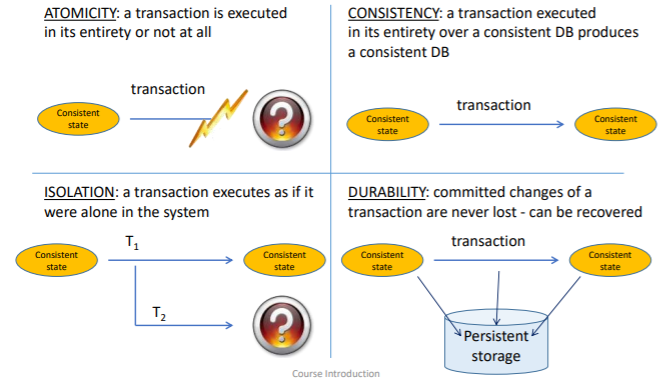
\includegraphics[scale=0.8]{images/00-acid.PNG}
	\caption{The ACID principle.}
	\label{fig:acid}
\end{figure}

\paragraph{Basic Database Architectures}
Shared nothing: each node runs its own data and its own engine, they share neither disk nor memory. Needs function shipping (query has to go where the data is) and / or data shipping (data has to go where query is). Easy to maintain and to scale, ideal when data can be partitioned / replicated and updates are not frequent. Shared memory: a coherent memory abstraction is provided over the network, merging the memory of each node, allowing for easier programming. Shared disk: data is stored in shared storage with a network typically attached to it, needs data shipping. Very common for cloud architectures. Separates storage from compute.

\subsection{Reading Assignments}

\subsubsection{Architecture of a Database System}

\subsection{Exercises}

\subsubsection{Introductory Topics}